\documentclass[10pt]{article}
\usepackage[utf8]{inputenc}
\usepackage{amsmath}
\usepackage{amssymb}
\usepackage{graphicx}
\usepackage{geometry}
\usepackage{enumitem}
\usepackage{multicol}
\usepackage{ifthen}
\usepackage[american]{circuitikz}
\usepackage{pgfplots}
\pgfplotsset{compat=1.18}
\geometry{a4paper, margin=1in}

\pagestyle{empty} % Completely remove page numbers

\title{\vspace{-1.5cm}\Large\textbf{University of Nebraska-Lincoln}\\[0.2cm]
\Large\textbf{Electronic Circuits: Quiz 3}}
\date{\vspace{-0.5cm}\small\textbf{February 20, 2026}} 

\newboolean{showresults}
\setboolean{showresults}{false}

\begin{document}

\maketitle

\noindent\textbf{Name:} \underline{\hspace{10cm}} \hfill \textbf{Total Points: 10}


% \vspace{0.5cm}

% \noindent\textbf{Useful Equations:}
% \[
% R = \frac{V}{I}, \quad r = \frac{dV}{dI}
% \]

\vspace{0.3cm}

\begin{enumerate}
    \item \textbf{(5 points)} The figure below shows the current-voltage (I-V) characteristics for three different resistors.
    
    \begin{center}
    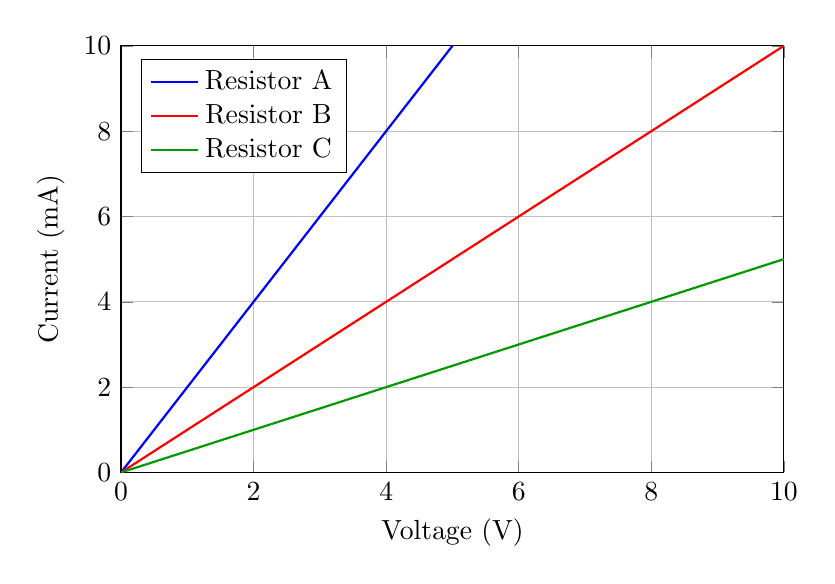
\begin{tikzpicture}
        \begin{axis}[
            width=10cm,
            height=7cm,
            xlabel={Voltage (V)},
            ylabel={Current (mA)},
            xmin=0, xmax=10,
            ymin=0, ymax=10,
            grid=major,
            legend pos=north west,
            ]
            % Resistor 1: R = 500 Ω (steepest slope)
            \addplot[blue, thick, domain=0:10] {x/0.5};
            \addlegendentry{Resistor A}
            
            % Resistor 2: R = 1000 Ω (medium slope)
            \addplot[red, thick, domain=0:10] {x/1};
            \addlegendentry{Resistor B}
            
            % Resistor 3: R = 2000 Ω (shallowest slope)
            \addplot[green!60!black, thick, domain=0:10] {x/2};
            \addlegendentry{Resistor C}
        \end{axis}
    \end{tikzpicture}
    \end{center}
    
    \textbf{Which resistor has the highest resistance and why?}
    
    % \begin{enumerate}[label=(\Alph*)]
    %     \item Resistor A, because it has the steepest slope
    %     \item Resistor B, because it is in the middle
    %     \item Resistor C, because it has the shallowest slope
    %     \item All resistors have the same resistance
    % \end{enumerate}
    
    % \vspace{0.5cm}
    
    \ifthenelse{\boolean{showresults}}{
        \textbf{Solution:}
        
        \textbf{Answer: (C) Resistor C, because it has the shallowest slope}
        
        For a linear resistor, resistance is given by $R = V/I$, which is the inverse of the slope in an I-V plot. The resistor with the shallowest slope (smallest $\Delta I/\Delta V$) has the highest resistance. Resistor C requires more voltage to produce the same current compared to the other resistors, indicating it has the highest resistance.
        
    }{}
    
    % \newpage
    
    \item \textbf{(5 points)} The figure below shows the current-voltage (I-V) characteristic of a diode with three operating points marked as A, B, and C.
    
    \begin{center}
    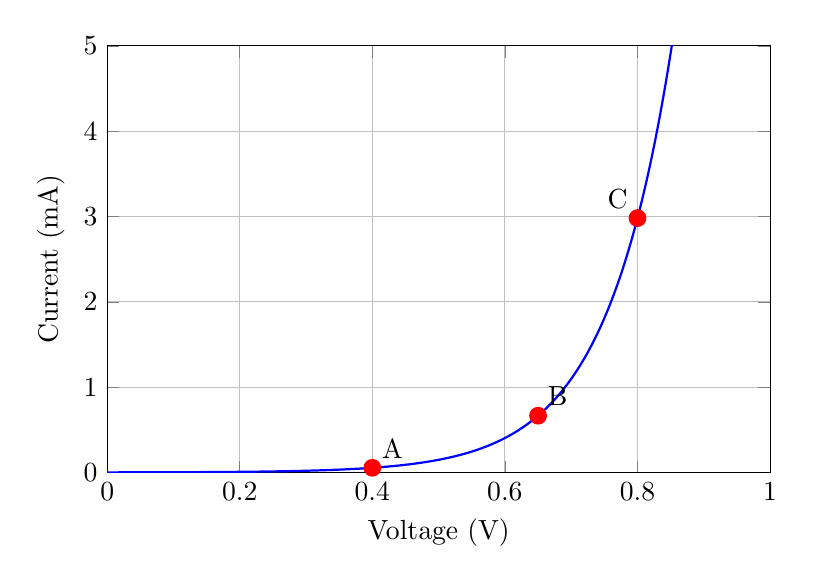
\begin{tikzpicture}
        \begin{axis}[
            width=10cm,
            height=7cm,
            xlabel={Voltage (V)},
            ylabel={Current (mA)},
            xmin=0, xmax=1.0,
            ymin=0, ymax=5,
            grid=major,
            ]
            % Diode exponential curve: I = Is*(exp(V/Vt) - 1)
            % Using simplified exponential: I ≈ 0.001*exp(10*V) for realistic diode behavior
            \addplot[blue, thick, smooth, samples=200, domain=0:0.9] {0.001*exp(10*x)};
            
            % Mark three points
            % Point A: V = 0.4V, low current region (shallowest tangent)
            \addplot[only marks, mark=*, mark size=3pt, red] coordinates {(0.4, {0.001*exp(10*0.4)})};
            \node[above right] at (axis cs:0.4,{0.001*exp(10*0.4)}) {A};
            
            % Point B: V = 0.65V, medium current region
            \addplot[only marks, mark=*, mark size=3pt, red] coordinates {(0.65, {0.001*exp(10*0.65)})};
            \node[above right] at (axis cs:0.65,{0.001*exp(10*0.65)}) {B};
            
            % Point C: V = 0.8V, high current region (steepest tangent)
            \addplot[only marks, mark=*, mark size=3pt, red] coordinates {(0.8, {0.001*exp(10*0.8)})};
            \node[above left] at (axis cs:0.8,{0.001*exp(10*0.8)}) {C};
        \end{axis}
    \end{tikzpicture}
    \end{center}
    
    \textbf{Which operating point has the highest small-signal resistance and why?}
    
    % \begin{enumerate}[label=(\Alph*)]
    %     \item Point A, because it has the steepest tangent slope at that point
    %     \item Point A, because it has the shallowest tangent slope at that point
    %     \item Point C, because it has the steepest tangent slope at that point
    %     \item Point C, because it has the shallowest tangent slope at that point
    % \end{enumerate}
    
    \vspace{0.5cm}
    
    \ifthenelse{\boolean{showresults}}{
        \textbf{Solution:}
        
        \textbf{Answer: (B) Point A, because it has the shallowest tangent slope at that point}
        
        The small-signal resistance (also called dynamic or incremental resistance) is defined as $r = dV/dI$, which is the inverse of the slope of the tangent line to the I-V curve at the operating point. Point A is in the lower current region where the exponential curve is less steep, meaning $dI/dV$ is smaller, and therefore $r = dV/dI$ is larger. As the diode current increases (moving from A to B to C), the curve becomes steeper, the tangent slope increases, and the small-signal resistance decreases.
        
    }{}
    
\end{enumerate}

\end{document}
